\clearpage

\section{Supersolidity in the V Phase}\label{sec-nbcp-v-phase}

The pure-PD limit has an additional exact spin symmetry that changes the
allowed angular anisotropy of the V state. At \(J_\Gamma=0\), a common
spin rotation by \(\pi\) leaves the microscopic Hamiltonian invariant.
Together with the threefold operation on the V orbit, this forbids a
threefold pinning term and permits sixfold pinning. The saved
zero-point-energy scans exhibit precisely this distinction: sixfold
modulation for pure PD and threefold modulation for pure \(\Gamma\).

This is a qualification of the finite-temperature argument, not a
demonstration of a thermal V supersolid. A nonzero zero-temperature
pseudo-Goldstone gap is compatible with an intermediate algebraic phase
when the clock anisotropy is irrelevant there. Whether that phase occurs
in this microscopic model also depends on its stiffness, defects and
competing orders.

\subsection{The claim being examined}\label{the-claim-being-examined}

Park et al.~\cite{park2026} use sixfold and threefold clock descriptions for Y
and V, respectively, in Eqs. (3) and (4). Their thermal argument permits
an intermediate BKT regime for Y and excludes it for V. The symmetry
analysis in Section~\ref{sec-nbcp-v-symmetry} distinguishes PD from
\(\Gamma\) through a spin-only \(\pi\) rotation. The present review asks
how the thermal conclusion must be scoped on the exactly \(J_\Gamma=0\)
axis.

The reference state, exchange conventions, fields and energy
normalization are those of the \hyperref[sec-nbcp-gap-appendix]{Y/V
curvature note}. The angular variable \(\phi\) is the same physical
global-\(z\) rotation, with period \(2\pi\). The derivation below
follows one three-sublattice domain and does not identify the full
manifold, including translation domains, with a single clock variable.

\subsection{The extra symmetry at zero Gamma
coupling}\label{sec-nbcp-v-symmetry}

Under \(R_z(\pi)\), the spin components transform as

\[
(\hat S^x,\hat S^y,\hat S^z)\longmapsto(-\hat S^x,-\hat S^y,\hat S^z).
\]

The XXZ terms, longitudinal Zeeman term and PD terms contain an even
number of transverse spin components. Each \(\Gamma\) term contains one
transverse component and one longitudinal component. Consequently,
rotation of every spin maps the family of Hamiltonians according to

\[
\hat U_\pi\hat H(J_{\rm PD},J_\Gamma)\hat U_\pi^\dagger
=\hat H(J_{\rm PD},-J_\Gamma).
\]

Only at \(J_\Gamma=0\) is this a symmetry of the same generic PD
Hamiltonian. An effective angular energy or free energy that preserves
this exact microscopic symmetry must then satisfy

\[
v(\phi+\pi)=v(\phi).
\]

For the V configuration, the combined lattice-spin threefold operation
preserves the equivalent pair of sublattices and shifts the orbit
coordinate by \(2\pi/3\), up to its sign convention. Thus

\[
v(\phi+2\pi/3)=v(\phi).
\]

Write a real angular potential as

\[
v(\phi)=v_0+\sum_{n\ge1}\bigl[a_n\cos(n\phi)+b_n\sin(n\phi)\bigr].
\]

The first symmetry requires even \(n\) and the second requires
\(n\in3\mathbb Z\). Their intersection is \(n\in6\mathbb Z\), so the
leading symmetry-allowed potential on the pure-PD V branch is

\[
v_{\rm V}^{\rm PD}(\phi)
=v_0-\lambda_6\cos(6\phi-\delta_6)+\text{higher multiples of six}.
\]

This statement does not require a nonzero \(\lambda_6\) at every
parameter point. At the representative point below, the sixfold
coefficient is nonzero. At generic nonzero \(J_\Gamma\), the spin-only
\(\pi\) symmetry is lost and a term \(-\lambda_3\cos(3\phi-\delta_3)\)
is allowed. Its lowest orders are \(J_{\rm PD}J_\Gamma\) and
\(J_\Gamma^3\) (Section~\nbcpnoteref{Y/V low energy and pseudo-Goldstone gap}{``Order of the angular harmonics in the SOC couplings''}). The phase offsets \(\delta_p\) specify the origin of
\(\phi\) and do not change the harmonic order.

\subsection{Numerical evidence without a symmetry-constrained
fit}\label{numerical-evidence-without-a-symmetry-constrained-fit}

The diagnostic reanalyzes the saved \(T=0\) energies at \(S=1/2\),
\(J=0.075\) meV and \(J_z=0.125\) meV. The fields are \(B=0.2\) T for Y
and \(B=1.4\) T for V. Exactly one SOC coupling is \(0.010\) meV in each
row. With \(M=72\) uniformly spaced angles and
\(\bar e=M^{-1}\sum_j e_j\), the discrete coefficients are

\[
c_n=\frac{2}{M}\sum_{j=0}^{M-1}(e_j-\bar e)e^{-\mathrm i n\phi_j},
\qquad A_n=|c_n|=\sqrt{a_n^2+b_n^2}.
\]

All sampled harmonics below the Nyquist mode are evaluated. No threefold
or sixfold selection rule is imposed. At base mesh \(N=48\), the
amplitudes are:

\begin{longtable}[]{@{}
  >{\raggedright\arraybackslash}p{(\linewidth - 8\tabcolsep) * \real{0.1667}}
  >{\raggedright\arraybackslash}p{(\linewidth - 8\tabcolsep) * \real{0.1667}}
  >{\raggedleft\arraybackslash}p{(\linewidth - 8\tabcolsep) * \real{0.2222}}
  >{\raggedleft\arraybackslash}p{(\linewidth - 8\tabcolsep) * \real{0.2222}}
  >{\raggedleft\arraybackslash}p{(\linewidth - 8\tabcolsep) * \real{0.2222}}@{}}
\toprule\noalign{}
\begin{minipage}[b]{\linewidth}\raggedright
Phase
\end{minipage} & \begin{minipage}[b]{\linewidth}\raggedright
Nonzero coupling
\end{minipage} & \begin{minipage}[b]{\linewidth}\raggedleft
\(A_3\) (meV/spin)
\end{minipage} & \begin{minipage}[b]{\linewidth}\raggedleft
\(A_6\) (meV/spin)
\end{minipage} & \begin{minipage}[b]{\linewidth}\raggedleft
Dominant harmonic
\end{minipage} \\
\midrule\noalign{}
\endfirsthead
\toprule\noalign{}
\begin{minipage}[b]{\linewidth}\raggedright
Phase
\end{minipage} & \begin{minipage}[b]{\linewidth}\raggedright
Nonzero coupling
\end{minipage} & \begin{minipage}[b]{\linewidth}\raggedleft
\(A_3\) (meV/spin)
\end{minipage} & \begin{minipage}[b]{\linewidth}\raggedleft
\(A_6\) (meV/spin)
\end{minipage} & \begin{minipage}[b]{\linewidth}\raggedleft
Dominant harmonic
\end{minipage} \\
\midrule\noalign{}
\endhead
\bottomrule\noalign{}
\caption{Unconstrained angular-energy harmonics for the sampled Y and V states.}\label{tab-nbcp-08-v-phase-1}\\
\endlastfoot
Y & PD & \(7.19\times10^{-19}\) & \(1.4367745\times10^{-6}\) & 6 \\
Y & Gamma & \(1.93\times10^{-18}\) & \(1.6429350\times10^{-12}\) & 6 \\
V & PD & \(4.28\times10^{-19}\) & \(1.0239780\times10^{-5}\) & 6 \\
V & Gamma & \(7.1609759\times10^{-7}\) & \(8.9632094\times10^{-11}\) &
3 \\
\end{longtable}

The forbidden threefold amplitudes are at the scale of numerical noise;
the exact vanishing follows from symmetry, not from declaring those
fitted numbers to be zero. The same dominant harmonic is obtained from
the \(N=12\) and \(N=24\) saved scans. For pure-PD V, the largest
sampled difference \(|e(\phi+\pi/3)-e(\phi)|\) is \(2.35\times10^{-17}\)
meV/spin or less at \(N=48\). With pure \(\Gamma\), that difference
reaches \(1.4322\times10^{-6}\) meV/spin, whereas the \(2\pi/3\) shift
remains invariant to numerical precision.

\begin{figure}

\centering{

\nbcpbounded{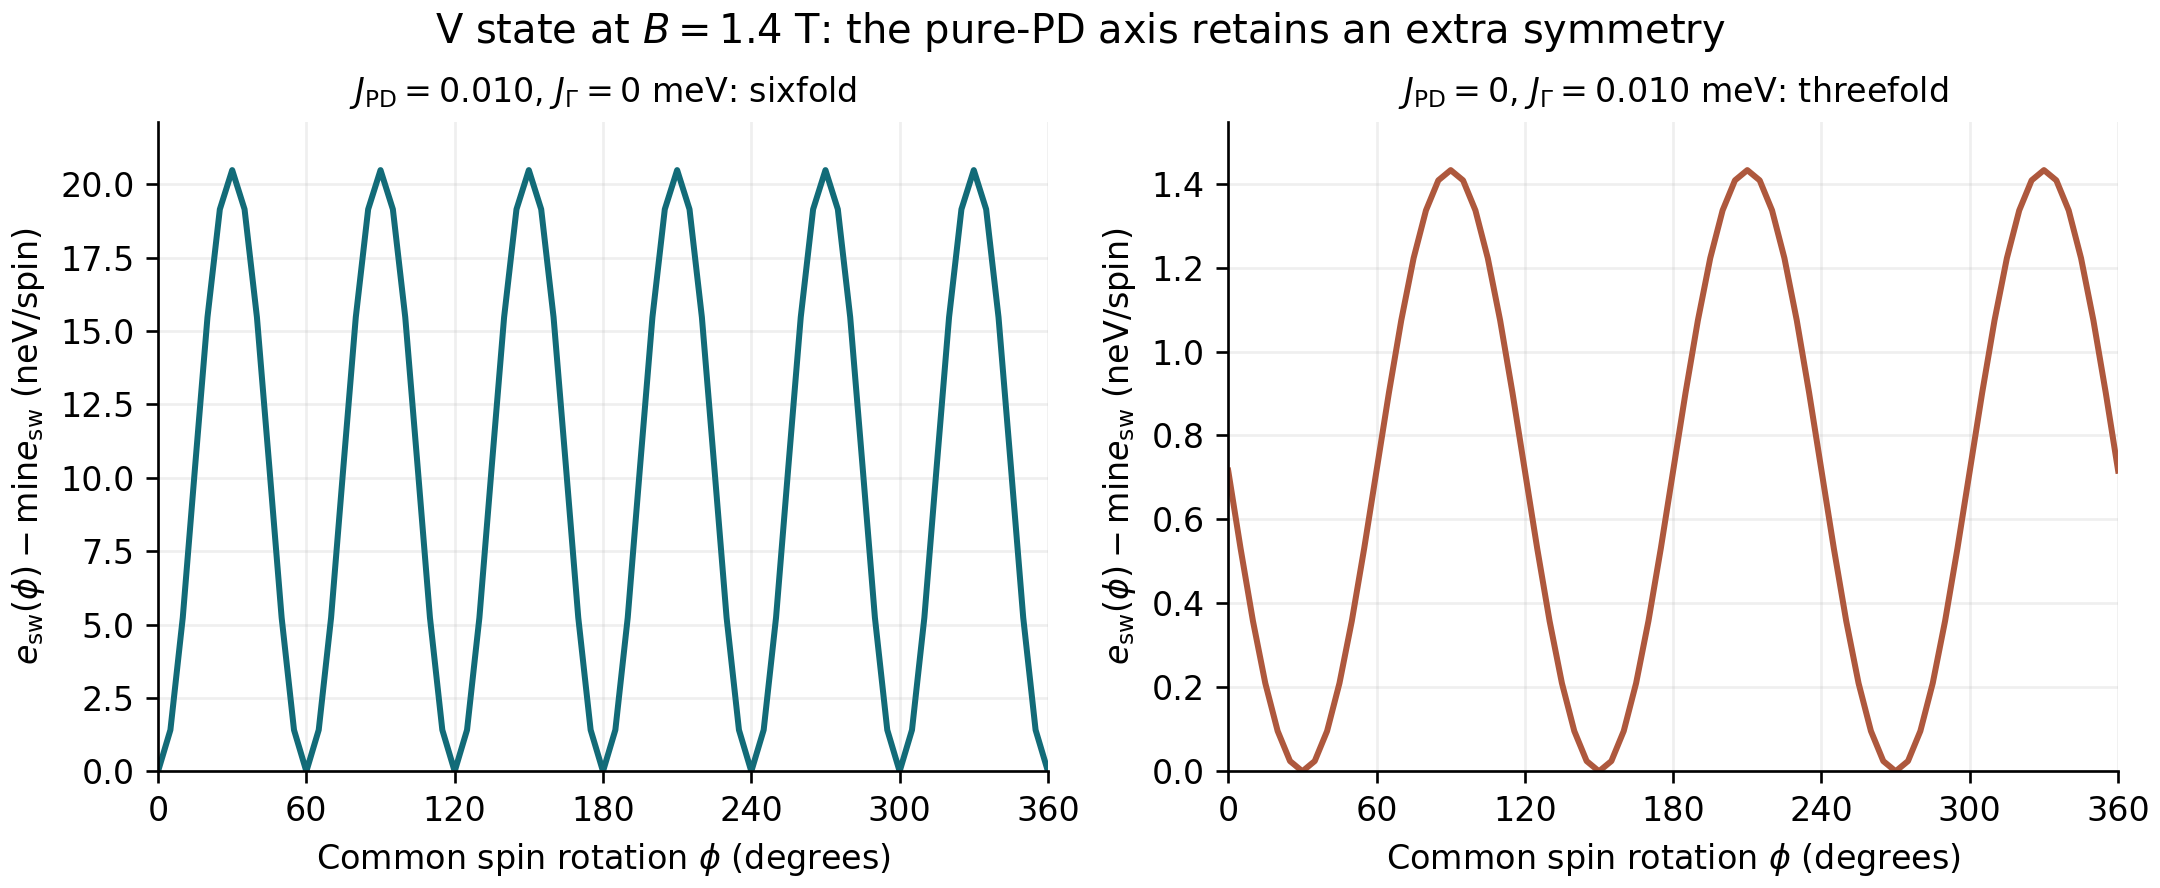
\includegraphics[keepaspectratio]{figures/v-clock-anisotropy.png}}

}

\caption{\label{fig-nbcp-clock}The V-state zero-point energy along the
common global-z orbit. Pure PD produces six minima while pure Gamma
produces three. Each panel uses absolute energy differences per physical
spin, with its own vertical scale; the curves are not normalized by
their angular ranges.}

\end{figure}%

The saved Brillouin-zone quadrature includes rotated momentum copies. To
check that the pure-PD result is not solely a consequence of that
averaging, an additional calculation uses Cartesian Holstein-Primakoff
matrices at 128 fresh, unsymmetrized momenta and \(\phi=0.173\) rad. For
pure-PD V, the largest matrix difference after \(\phi\mapsto\phi+\pi\)
is \(2.87\times10^{-17}\) meV. The individual exchange matrices obey
\(R_z(\pi)^\mathsf T\mathsf J R_z(\pi)=\mathsf J\) exactly in
floating-point arithmetic. For nonzero \(\Gamma\), the corresponding
test passes only after also reversing \(J_\Gamma\), with a maximum
matrix residual below \(2.9\times10^{-17}\) meV across the four
representative cases.

These checks share the existing bond geometry and state inputs. They
support the stated symmetry identities; they are not an independent
microscopic-model reconstruction or a finite-temperature calculation.
Finite angular sampling can alias higher harmonics, so the table alone
is not an all-orders Fourier theorem.

\subsection{Higher harmonics and threefold pinning near the PD
axis}\label{sec-nbcp-v-mixed-soc}

\textbf{Twelfth harmonic on the PD axis.} The saved \(N=48\) V scan at
\(J_{\rm PD}=0.010\) meV has \(\lambda_{12}/\lambda_6=7.31\times10^{-3}\)
and \(\lambda_{18}/\lambda_6=9.0\times10^{-5}\). Because the curvature
weights the \(n\)th amplitude by \(n^2\), the resolved minimum curvature
exceeds \(36\lambda_6\) by 3.0\%, compared with 1.14\% for Y at the same
coupling (Section~\nbcpnoteref{Y phase supersolidity}{``Angular matching of Y stiffness and potential''}). The V/PD gap in
Section~\nbcpnoteref{Y/V low energy and pseudo-Goldstone gap}{``Numerical comparison''} already uses the resolved curvature; a
sixth-only clock potential would underestimate it by about 1.5\%.

\textbf{Mixed couplings.} The selection rule of
Section~\nbcpnoteref{Y/V low energy and pseudo-Goldstone gap}{``Order of the angular harmonics in the SOC couplings''} allows a threefold V harmonic at
order \(J_{\rm PD}J_\Gamma\). To test it, the vacuum energy is evaluated on
the fixed classical V orbit at \(B=1.4\) T for \(J_{\rm PD}=0\), 0.005 and
0.010 meV and \(J_\Gamma=0.00025\)--0.002 meV, with 72 angles and base
mesh \(N=24\). On the pure axes, \(N=24\) and \(N=48\) gaps differ by less
than \(10^{-4}\) relatively (Section~\nbcpnoteref{Numerical verification and provenance}{``Numerical convergence''}). The Fourier
amplitudes are extracted without imposing a selection rule.

\begin{longtable}[]{@{}rrrrrrr@{}}
\toprule\noalign{}
\(J_{\rm PD}\) & \(J_\Gamma\) & \(\lambda_3\) & \(\lambda_6\) &
\(\lambda_3/(J_{\rm PD}J_\Gamma)\) & \(r\) & \(\Delta_{\rm PG}\) \\
\midrule\noalign{}
\endfirsthead
\toprule\noalign{}
\(J_{\rm PD}\) & \(J_\Gamma\) & \(\lambda_3\) & \(\lambda_6\) &
\(\lambda_3/(J_{\rm PD}J_\Gamma)\) & \(r\) & \(\Delta_{\rm PG}\) \\
\midrule\noalign{}
\endhead
\bottomrule\noalign{}
\caption{Threefold and sixfold V harmonics near the PD axis at 1.4 T.
Couplings and gaps in meV, amplitudes in meV/spin, the ratio in
meV\(^{-1}\); \(r=\lambda_3/(4\lambda_6)\).}\label{tab-nbcp-v-mixed-soc}\\
\endlastfoot
0.005 & 0.00025 & \(1.712\times10^{-6}\) & \(7.297\times10^{-7}\) & 1.3692 & 0.586 & 0.00334 \\
0.005 & 0.00050 & \(3.423\times10^{-6}\) & \(7.292\times10^{-7}\) & 1.3693 & 1.174 & 0.00171 \\
0.005 & 0.00100 & \(6.848\times10^{-6}\) & \(7.272\times10^{-7}\) & 1.3696 & 2.354 & 0.00477 \\
0.005 & 0.00200 & \(1.371\times10^{-5}\) & \(7.193\times10^{-7}\) & 1.3706 & 4.764 & 0.00792 \\
0.010 & 0.00025 & \(4.574\times10^{-6}\) & \(1.024\times10^{-5}\) & 1.8295 & 0.112 & 0.01554 \\
0.010 & 0.00050 & \(9.148\times10^{-6}\) & \(1.023\times10^{-5}\) & 1.8296 & 0.224 & 0.01523 \\
0.010 & 0.00100 & \(1.830\times10^{-5}\) & \(1.021\times10^{-5}\) & 1.8302 & 0.448 & 0.01392 \\
0.010 & 0.00200 & \(3.665\times10^{-5}\) & \(1.013\times10^{-5}\) & 1.8326 & 0.905 & 0.00666 \\
\end{longtable}

At fixed \(J_{\rm PD}\), a log-log fit of \(\lambda_3\) against
\(J_\Gamma\) gives slopes 1.0005 and 1.0008, while the pure-Gamma points
give 3.0004. Reversing \(J_\Gamma\) at \(J_{\rm PD}=0.010\) meV leaves
\(\lambda_3\) unchanged and shifts its phase by \(\pi\), so the coefficient
is odd in \(J_\Gamma\) as required. The ratio
\(\lambda_3/(J_{\rm PD}J_\Gamma)\) is 1.369 meV\(^{-1}\) at
\(J_{\rm PD}=0.005\) meV and 1.830 meV\(^{-1}\) at 0.010 meV. Its
dependence on \(J_{\rm PD}\) shows a sizable \(J_{\rm PD}^2J_\Gamma\)
contribution, which the rule also allows; as for the sixfold harmonic,
these points are not in the asymptotic weak-SOC regime.

\textbf{Competition and leading-order gap closing.} The fitted phases
place the threefold minima exactly at maxima of the sixfold term. The
calculated energy is also symmetric under reflection of the angle about
\(\phi=\pi/6\) to within \(2\times10^{-17}\) meV/spin. This follows from
the antiunitary \(C_2'\mathcal T\) of
Section~\nbcpnoteref{NBCP model and phase diagram}{``Symmetries''}. It keeps the
longitudinal field and every sublattice label and maps the V orbit point
\(\phi\) to \(\pi-\phi\) at the same polar angles, so
\(v(\phi)=v(\pi-\phi)\). The threefold operation adds the period
\(2\pi/3\), so the reflection centres are \(\pi/2+m\pi/3\), which include
\(\pi/6\). A reflection about \(\phi=0\) is not implied. A direct check
with mixed \(J_{\rm PD}\) and either sign of \(J_\Gamma\) finds the bond
matrices invariant to \(1.4\times10^{-17}\) meV and
\(v(\pi-\phi)-v(\phi)\) and \(v(\phi+2\pi/3)-v(\phi)\) below
\(2\times10^{-17}\) meV/spin. The control \(v(-\phi)-v(\phi)\) is instead
of order \(10^{-5}\) meV/spin. The map also forces the threefold phase
\(\delta_3\) to \(\pm\pi/2\), as found, so that
\(\cos(3\phi-\delta_3)=\pm\sin3\phi\). With these phases and only the two
harmonics,
\begin{equation}\label{eq-nbcp-v-mixed-curvature}
C_\phi=\begin{cases}
36\lambda_6(1-r^2), & r<1,\\
9\lambda_3-36\lambda_6, & r>1,
\end{cases}
\qquad r=\frac{\lambda_3}{4\lambda_6}.
\end{equation}
For \(r<1\), six degenerate minima related by the threefold operation and
the reflection move away from the sixfold minima. At \(r=1\), pairs of
them merge at the three threefold minima. This expression reproduces the
resolved curvatures within the size of the higher harmonics. The
leading-order gap therefore first decreases and then reopens as
\(J_\Gamma\) grows. Extrapolating the smallest-\(J_\Gamma\) slopes, \(r=1\)
occurs near \(J_\Gamma\approx0.0004\) meV for \(J_{\rm PD}=0.005\) meV and
near 0.0022 meV for \(J_{\rm PD}=0.010\) meV, that is at
\(J_\Gamma/J_{\rm PD}\approx0.09\) and 0.22. At that point the quadratic
pinning vanishes and the leading-order gap is zero; the actual gap is set
by quartic angular terms and higher-order corrections not computed here.
It is therefore not assigned a physical value.

For the thermal argument, the threefold amplitude is a relevant
perturbation at the Gaussian line throughout the sixfold window, since
its eigenvalue \(2-9/(4\pi K)\) is positive for every \(K>2/\pi\). The
selection rule makes that amplitude linear in \(J_\Gamma\) near the PD
axis, so the pure-PD sixfold scenario is not protected against a small
Gamma coupling. Which finite-temperature sequence of phases follows when
six degenerate minima carry unequal barriers has not been analyzed.

\subsection{Local gap and missing spatial
matching}\label{local-gap-and-missing-spatial-matching}

The V canonical response and representative zero-temperature gaps are
recorded in Section~\nbcpnoteref{Y/V low energy and pseudo-Goldstone gap}{``Y and V states''} and Section~\nbcpnoteref{Y/V low energy and pseudo-Goldstone gap}{``Numerical comparison''}. They
establish a local curvature comparison under the conditions of
Section~\nbcpnoteref{Y/V low energy and pseudo-Goldstone gap}{``Approximation and interpretation''}. The sixfold potential on the pure-PD
axis changes the symmetry-based thermal question, but the V stiffness,
defect weights and thermal RG initial conditions have not been matched.
The Y gradient and wall results cannot be transferred to V without
repeating those phase-specific calculations.
